\documentclass{book}

\usepackage[utf8]{inputenc}
\usepackage[frenchb]{babel}
\usepackage{lipsum}
\usepackage{graphicx}

% permet de faire une table des matieres par chapitre
\usepackage[french]{minitoc}

% ajoute (entre autre) la bibliographie dans la table des matieres 
\usepackage[nottoc]{tocbibind}

% biblio ordonnee classique
\bibliographystyle{unsrt}
\title{Exemple de thèse \LaTeX{} qui se veut minimal}
\author{G. Vallverdu}
\date{\today}

\begin{document}

% le titre
\maketitle

% preparation des minitocs
\dominitoc

% table des matieres generale
\tableofcontents

% inclusion des chapitres
\chapter*{Introduction}
% pour faire apparaitre l'introduction dans le sommaire et que les minitocs soient au bon
% endroit
\addstarredchapter{Introduction générale} 

% Pour que l'entete soit correcte car chapter* ne redefinit pas l'entete.
\markboth{INTRODUCTION}{}

\lipsum[22-26]



\chapter{Premier chapitre}

\minitoc

\section{Citations}

Ici on cite un article de Dudarev\cite{Dudarev1998}, puis un sur Bader\cite{Henkelman2006}
et un petit dernier\cite{Blochl1994}. Le tout pour tester la bibliographie par chapitre.

\lipsum[6-8]

\section{Paragraphe}

\lipsum[9-12]



\section{Humanités numériques et lettres classiques}
\label{sec:digitalclassics}

\subsection{Introduction}
\label{subsec:dc_intro}

Relation HN et DigiClass (// Annales et LC ?)

\subsection{Production de corpus}
\label{subsec:dc_histoirecorpus}

Histoire de ..

\subsection{Analyse de la langue}
\label{subsec:dc_langue}

Histoire de ..



\section{Corpus}
\label{sec:corpus}

\subsection{Constitution, sources du corpus}
\label{subsec:corpus_constitution}

\subsection{Répartition chronologique du corpus}
\label{subsec:corpus_chrono}

\begin{figure}[h]
    \centering
    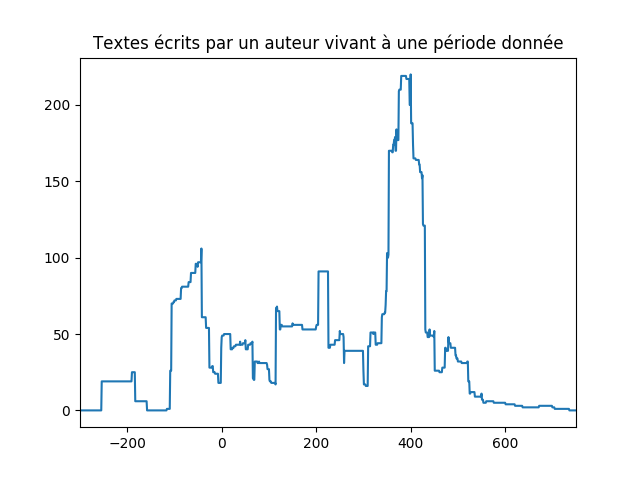
\includegraphics[width=10cm]{../results/analysis/corpus_analysis/texts_per_year.png}
    \caption{Répartition des textes en fonction de l'année de naissance et de mort de l'auteur}
    \label{texts_per_year}
\end{figure}

\begin{figure}[h]
    \centering
    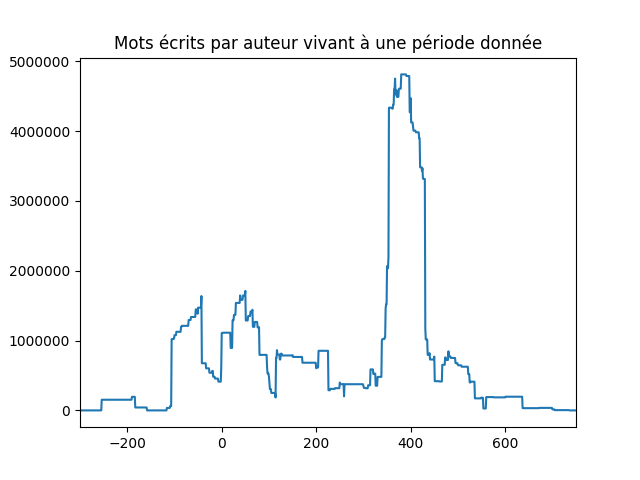
\includegraphics[width=10cm]{../results/analysis/corpus_analysis/tokens_per_year.png}
    \caption{Répartition des mots en fonction de l'année de naissance et de mort de l'auteur}
    \label{tokens_per_year}
\end{figure}

\begin{figure}[h]
    \centering
    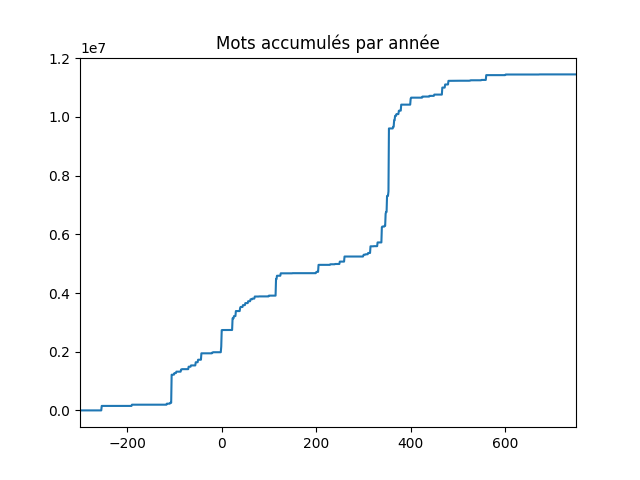
\includegraphics[width=10cm]{../results/analysis/corpus_analysis/accumulated_tokens.png}
    \caption{Nombre de mots accumulés au fil des années}
    \label{accumulated_tokens_per_year}
\end{figure}


\paragraph{Méthodes de datation}

\subsection{Découpage du corpus}
\label{subsec:corpus_decoupage}

\begin{figure}[h]
    \centering
    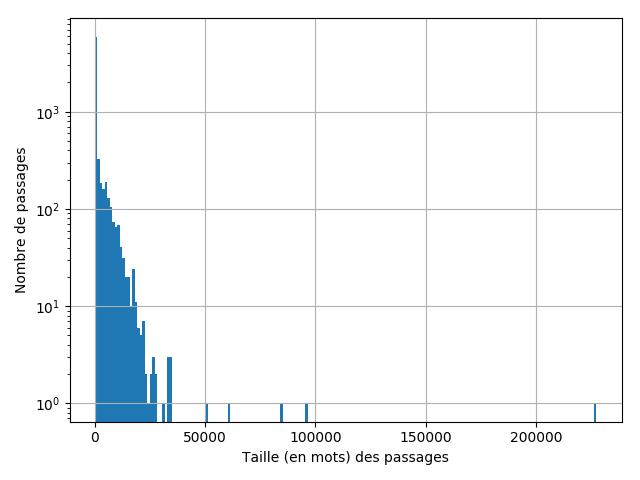
\includegraphics[width=10cm]{../results/analysis/corpus_analysis/passage_size_distribution.png}
    \caption{Répartition des tailles (en mots) d'extraits}
    \label{passage_size_distribution}
\end{figure}

\subsection{Statistiques lexicales du corpus}
\label{subsec:corpus_lexical_stats}

\subsection{Risques de répétition : analyse des doublons}
\label{subsec:corpus_repetition}

Basé sur l'étude de l'impact des duplications de texte en topic modeling \cite{schofield2017quantifying}, nous proposons ici une expérience
quant à la nécessité pour le corpus d'être soigné.
\section{Traitement automatique du latin : la lemmatisation}
\label{sec:lemmatiseurs}

\subsection{Introduction}
\label{subsec:lemma_intro}

Description des différentes tâches :
POS, Morph,

\subsection{Les analyseurs morphologiques}
\label{subsec:lemma_morph}

Collatinus, LatMor, etc.

\subsection{Les lemmatiseurs}
\label{subsec:lemma_lemmatiseurs}

Pandora, TreeTagger, etc.


\subsection{Corpus de test et méthode d'évaluation}
\label{subsec:lemma_corpus}

Détail sur le corpus de test

\subsection{Analyse des résultats}
\label{subsec:lemma_resultats}


\chapter{Second chapitre}

\minitoc

\section{Citations}

On remet une petite couche de biblio\cite{Kresse1993}. Toujours pour voir si la
bibliographie est bien par chapitre\cite{Kresse1996}.

\lipsum[13-16]

\section{Texte}

\lipsum[17-21]



\chapter*{Conclusion}
% pour faire apparaitre l'introduction dans le sommaire
\addcontentsline{toc}{chapter}{Conclusion}

% Pour que l'entete soit correcte car chapter* ne redefinit pas l'entete.
\markboth{CONCLUSION}{}

\lipsum[22-25]



\appendix

\chapter{Une annexe}

\lipsum[26-27]



% bibliographie
\bibliography{allbiblio}

\end{document}

